% *********************************************************************
% © 2021–2026 Jeremy Sylvestre
%
% Permission is granted to copy, distribute and/or modify this document
% under the terms of the GNU Free Documentation License, Version 1.3 or
% any later version published by the Free Software Foundation; with no
% Invariant Sections, no Front-Cover Texts, and no Back-Cover Texts. A
% copy of the license is included in the appendix entitled “GNU Free
% Documentation License” that appears in the output document of this
% PreTeXt source code. All trademarks™ are the registered® marks of
% their respective owners.
%
% *********************************************************************

\newcommand*{\xmin}{-6}
\newcommand*{\xmax}{42}
\newcommand*{\ymin}{-10}
\newcommand*{\ymax}{110}

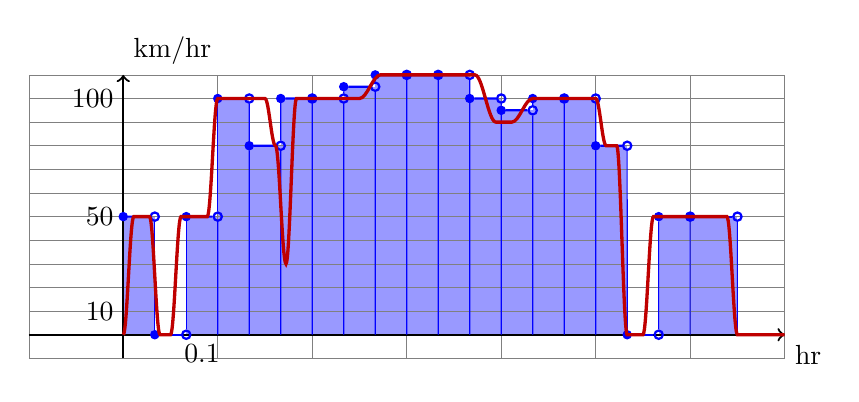
\begin{tikzpicture}
[
	closedpt/.style={circle,draw,fill,inner sep=0pt,minimum size=3pt},
	openpt/.style={circle,draw,inner sep=0pt,minimum size=3pt},
	xscale=0.2,
	yscale=0.03
]

	% rectangle fills
	% camrose
	\fill[blue!40!white] (0,50) rectangle (2,0);
	% 0-height rect
	\fill[blue!40!white] (4,50) rectangle (6,0);
	% highway 1
	\fill[blue!40!white] (6,100) rectangle (8,0);
	\fill[blue!40!white] (8,80) rectangle (10,0);
	\fill[blue!40!white] (10,100) rectangle (12,0);
	% highway 2
	\fill[blue!40!white] (12,100) rectangle (14,0);
	\fill[blue!40!white] (14,105) rectangle (16,0);
	\fill[blue!40!white] (16,110) rectangle (18,0);
	% highway 3
	\fill[blue!40!white] (18,110) rectangle (20,0);
	\fill[blue!40!white] (20,110) rectangle (22,0);
	\fill[blue!40!white] (22,100) rectangle (24,0);
	% highway 4
	\fill[blue!40!white] (24,95) rectangle (26,0);
	\fill[blue!40!white] (26,100) rectangle (28,0);
	\fill[blue!40!white] (28,100) rectangle (30,0);
	% wetaskiwin 1
	\fill[blue!40!white] (30,80) rectangle (32,0);
	% 0-height rect
	\fill[blue!40!white] (34,50) rectangle (36,0);
	% wetaskiwin 2
	\fill[blue!40!white] (36,50) rectangle (39,0);

	% grid
	\foreach \x in {-6,0,6,...,42} {
		\draw[very thin,gray] (\x,\ymin) -- (\x,\ymax);
	}
	\foreach \y in {-10,0,10,...,110} {
		\draw[very thin,gray] (\xmin,\y) -- (\xmax,\y);
	}

	% label grid
	\node[below] at (5,0) {$0.1$};

	\foreach \y in {10,50,100} {
		\node[left] at (0,\y) {$\y$};
	}

	% axes
	\draw[->,thick] (\xmin,0) -- (\xmax,0) node[below right] {hr};
	\draw[->,thick] (0,\ymin) -- (0,\ymax) node[above right] {$\mathrm{km}/\mathrm{hr}$};

	% Camrose
	\node[blue,closedpt] at (0,50) (cstart) {};
	\node[blue,thick,openpt] at (2,50) (cstop) {};
	\draw[blue,thick] (cstart) -- (cstop);
	\node[blue,closedpt] at (2,0) (cstart) {};
	\draw[blue,thin] (cstop) -- (cstart);
	\node[blue,thick,openpt] at (4,0) (cstop) {};
	\draw[blue,thick] (cstart) -- (cstop);
	\node[blue,closedpt] at (4,50) (cstart) {};
	\draw[blue,thin] (cstop) -- (cstart);
	\node[blue,thick,openpt] at (6,50) (cstop) {};
	\draw[blue,thick] (cstart) -- (cstop);
	\draw[blue,thin] (cstop) -- (6,0);

	% highway 1
	\node[blue,closedpt] at (6,100) (hstart) {};
	\draw[blue,thin] (cstop) -- (hstart);
	\node[blue,thick,openpt] at (8,100) (hstop) {};
	\draw[blue,thick] (hstart) -- (hstop);
	\node[blue,closedpt] at (8,80) (hstart) {};
	\draw[blue,thin]
	  (hstop) -- (hstart)
	  (hstart) -- (8,0)
	;
	\node[blue,thick,openpt] at (10,80) (hstop) {};
	\draw[blue,thick] (hstart) -- (hstop);
	\node[blue,closedpt] at (10,100) (hstart) {};
	\draw[blue,thin]
	  (hstop) -- (hstart)
	  (hstop) -- (10,0)
	;
	\node[blue,thick,openpt] at (12,100) (hstop) {};
	\draw[blue,thick] (hstart) -- (hstop);
	\draw[blue,thin] (hstop) -- (12,0);

	% highway 2
	\node[blue,closedpt] at (12,100) (hstart) {};
	\node[blue,thick,openpt] at (14,100) (hstop) {};
	\draw[blue,thick] (hstart) -- (hstop);
	\node[blue,closedpt] at (14,105) (hstart) {};
	\draw[blue,thin]
	  (hstop) -- (hstart)
	  (hstop) -- (14,0)
	;
	\node[blue,thick,openpt] at (16,105) (hstop) {};
	\draw[blue,thick] (hstart) -- (hstop);
	\node[blue,closedpt] at (16,110) (hstart) {};
	\draw[blue,thin]
	  (hstop) -- (hstart)
	  (hstop) -- (16,0)
	;
	\node[blue,thick,openpt] at (18,110) (hstop) {};
	\draw[blue,thick] (hstart) -- (hstop);
	\draw[blue,thin] (hstop) -- (18,0);

	% highway 3
	\node[blue,closedpt] at (18,110) (hstart) {};
	\node[blue,thick,openpt] at (20,110) (hstop) {};
	\draw[blue,thick] (hstart) -- (hstop);
	\draw[blue,thin] (hstop) -- (20,0);
	\node[blue,closedpt] at (20,110) (hstart) {};
	\node[blue,thick,openpt] at (22,110) (hstop) {};
	\draw[blue,thick] (hstart) -- (hstop);
	\node[blue,closedpt] at (22,100) (hstart) {};
	\draw[blue,thin]
	  (hstop) -- (hstart)
	  (hstart) -- (22,0)
	;
	\node[blue,thick,openpt] at (24,100) (hstop) {};
	\draw[blue,thick] (hstart) -- (hstop);

	% highway 3
	\node[blue,closedpt] at (24,95) (hstart) {};
	\draw[blue,thin]
	  (hstop) -- (hstart)
	  (hstart) -- (24,0)
	;
	\node[blue,thick,openpt] at (26,95) (hstop) {};
	\draw[blue,thick] (hstart) -- (hstop);
	\node[blue,closedpt] at (26,100) (hstart) {};
	\draw[blue,thin]
	  (hstop) -- (hstart)
	  (hstop) -- (26,0)
	;
	\node[blue,thick,openpt] at (28,100) (hstop) {};
	\draw[blue,thick] (hstart) -- (hstop);
	\draw[blue,thin] (hstop) -- (28,0);
	\node[blue,closedpt] at (28,100) (hstart) {};
	\node[blue,thick,openpt] at (30,100) (hstop) {};
	\draw[blue,thick] (hstart) -- (hstop);

	% Wetaskiwin 1
	\node[blue,closedpt] at (30,80) (wstart) {};
	\draw[blue,thin]
	  (hstop) -- (wstart)
	  (wstart) -- (30,0)
	;
	\node[blue,thick,openpt] at (32,80) (wstop) {};
	\draw[blue,thick] (wstart) -- (wstop);
	\draw[blue,thin] (wstop) -- (32,0);
	\node[blue,closedpt] at (32,0) (wstart) {};
	\node[blue,thick,openpt] at (34,0) (wstop) {};
	\draw[blue,thick] (wstart) -- (wstop);
	\node[blue,closedpt] at (34,50) (wstart) {};
	\draw[blue,thin] (wstop) -- (wstart);
	\node[blue,thick,openpt] at (36,50) (wstop) {};
	\draw[blue,thick] (wstart) -- (wstop);
	\draw[blue,thin] (wstop) -- (36,0);

	% Wetaskiwin 2
	\node[blue,closedpt] at (36,50) (wstart) {};
	\node[blue,thick,openpt] at (39,50) (wstop) {};
	\draw[blue,thick] (wstart) -- (wstop);
	\draw[blue,thin] (wstop) -- (39,0);

	% area divider
	% \draw[black,dashed]
	% 	(wstart) -- (0.5,0);
	% ;

	% continuous graph
	\draw[red!75!black,very thick]
	  (0,0)
	  cos ( 0.333,  25)
	  sin ( 0.667,  50)
	  --  ( 1.667,  50)
	  cos ( 2.000,  25)
	  sin ( 2.333,   0)
	  --  ( 3.000,   0)
	  cos ( 3.333,  25)
	  sin ( 3.667,  50)
	  --  ( 5.333,  50)
	  cos ( 5.667,  75)
	  sin ( 6.000, 100)
	  --  ( 9.000, 100)
	  cos ( 9.333,  90)
	  sin ( 9.667,  80)
	  cos (10.000,  55)
	  sin (10.333,  30)
	  cos (10.667,  65)
	  sin (11.000, 100)
	  --  (15.000, 100)
	  cos (15.667, 105)
	  sin (16.333, 110)
	  --  (22.333, 110)
	  cos (23.000, 100)
	  sin (23.667,  90)
	  --  (24.667,  90)
	  cos (25.333,  95)
	  sin (26.000, 100)
	  --  (30.000, 100)
	  cos (30.333,  90)
	  sin (30.667,  80)
	  --  (31.333,  80)
	  cos (31.667,  40)
	  sin (32.000,   0)
	  --  (33.000,   0)
	  cos (33.333,  25)
	  sin (33.667,  50)
	  --  (38.333,  50)
	  cos (38.667,  25)
	  sin (39.000,   0)
	  --  (\xmax,    0)
	;

\end{tikzpicture}
